\subsection{Design}

It was decided it would be in the best interests of the application if
real world data was used in the application as to properly demonstrate
the capabilities of the algorithm. A sensible starting source of data
was a text file containing the league standings and so a suitable data
source was created, based upon the American Baseball Season
2011-12.

Other alternatives were considered - mainly HTML or RSS parsing of
live scores. This was a suggestion to increase the user experience of
the application and to create a more immersive interaction between the
user and the application. Unfortunately, neither of these options
became a possibility due to the timing of the league and project
schedule - no baseball league was running during the time of the
project development and the risk was deemed too great to spend time
developing a parser for these sources when there is a chance no
suitable source could be found when the 2012-13 Season began.

Other sources of data were researched to see if an alternative sports
league could provide us with an active source and American Basketball
was a promising candidate. After much consideration of the scoring
system it was decided that anomalies occurred too frequently in
American Basketball which may give an unfair representation to
certain teams, and also to keep consistency throughout the rest of the
application - certain modules under development were reasonably
coupled to the league format already in place and it was decided
against changing this at such a late time in development.

Ultimately, the ability to immediately parse a full league was a major
benefit as it allowed the algorithm to become fully tested with a true
oracle at an earlier stage in development that the real-time parsing
would allow.

The parser is responsible for the instantiation of all league-related
objects required by all other parts of the application. At any stage,
the user should be able to change the league under examination to
another league with the same league format as the given one.

\subsection{Implementation}

The objects instantiated by the parser are:
\begin{itemize}
  \item[Division] This encapsulates the Teams belonging to a given
    Division, the list of Matches of the Teams in the Division and
    whether or not certain Matches have been played.
  \item[Match] Encapsulates a game between two Teams. Information
    stored is: Date played, Outcome of the game (if known) and the
    Date and Time the game is played on.
  \item[Team] Encapsulates information about a specific team: team
    Name, current Score and the teams Elimination Status amongst
    others.
\end{itemize}
\pagebreak
\begin{figure}[h]
  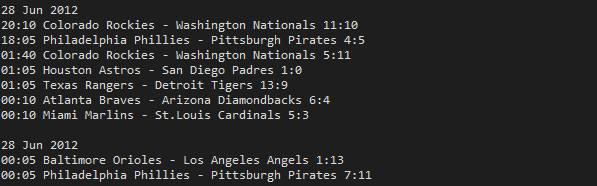
\includegraphics[width=\linewidth,keepaspectratio]{images/sourceFileExample.png}
  \caption{Sample data from the 2011-12 source file}\label{fig:BASESRC}
\end{figure}
\begin{figure}[h]
\begin{verbatim}
source
: days* EOF
;

days
: date EOL (match EOL)*
| EOL
;

date
: DAY MONTH YEAR
;

match
: TIME HOMETEAM HYPHEN AWAYTEAM HOMESCORE COLON AWAYSCORE
;
\end{verbatim}

\caption{Pseudo-grammar of the expected source file}\label{fig:GRAMMAR}
\end{figure}
As shown in Figure~\ref{fig:BASESRC}, the source file created follows
a standard format. The pseudo-grammar represented in
Figure~\ref{fig:GRAMMAR} where the tokens are:
\begin{itemize}
\item EOF -  End of file character
\item EOL - End of line character (`\textbackslash n')
\item DAY - The day on which the match was played
\item MONTH - The month in which the match was played
\item YEAR - The year in which the match was played
\item TIME - The time at which this game was played
\item HOMETEAM - The ``Home Team'' for this match
\item AWAYTEAM - The ``Away Team'' for this match
\item HOMESCORE - The ``Home Team''s score for this match
\item AWAYSCORE - The ``Away Team''s score for this match
\item HYPHEN - a literal ``-''
\item COLON - a literal ``:''
\end{itemize}

Using the pseudo-grammar the parser is now capable of instantiating
the objects required. It is of worth noting that to enforce separation
of concerns no data checking is done by the parser - this
responsibility is left to the object constructors. An error or warning
is raised however if information is missing and the element
responsible for this is discarded.

Prior to any parsing, the parser must be initialised with the league
information required by other modules of the application. This is hard
coded due to the coupling of other modules to an exact league format.

The pseudo-code in Algorithm~\ref{fig:PARSER} outlines the method in
which any source file is parsed.

\IncMargin{2em}
\begin{algorithm}
  \SetAlgoLined
  \SetKwData{Date}{Date} \SetKwData{Match}{Match}
  \SetKwData{File}{File} \SetKwData{Line}{Line}
  \SetKwData{Teams}{Teams} \SetKwData{Division}{Division}
  \SetKwInOut{Input}{input}

  \Input{A file \File to be parsed}
  \Date $\leftarrow$ a date object used in creating a \Match\;
  \Begin{
      \While{not at end of \File}{
        \Line $\leftarrow$ tokens of next line read from \File\;
        \uIf{\Line is a date}{
          \Date $\leftarrow$ extracted information from \Line\;
        }
        \uElseIf{\Line is a match}{
          \Match $\leftarrow$ extracted information about match from
          \Line\;
          date of \Match $\leftarrow$ \Date\;
          add \Match to upcoming games of the participating \Teams\;
          add \Match to fixtures of respective \Division\;
        }
        \Else{
          Badly formatted input, ignore\;
        }
      }
    }
    \caption{Parser}\label{fig:PARSER}
\end{algorithm}
\DecMargin{2em}


\clearpage
